\documentclass[10pt,a4paper]{article}
\usepackage{fontspec}
\usepackage{xeCJK}
\setmainfont{TeX Gyre Termes}
\setsansfont{TeX Gyre Heros}
\setmonofont{Latin Modern Mono}
\setCJKmainfont{Noto Serif CJK SC}
\setCJKsansfont{Noto Sans CJK SC}
\setCJKmonofont{Noto Sans Mono CJK SC}
\XeTeXlinebreaklocale "zh"
\XeTeXlinebreakskip = 0pt plus 1pt
\usepackage[a4paper,top=15mm,bottom=16mm,left=15mm,right=15mm]{geometry}
\usepackage{graphicx}
\usepackage{booktabs}
\usepackage{tabularx}
\usepackage{array}
\usepackage{amsmath,amssymb}
\usepackage{natbib}
\usepackage{xcolor}
\usepackage{hyperref}
\usepackage{caption}
\usepackage{titlesec}
\usepackage{enumitem}
\usepackage{dblfloatfix}
\usepackage{balance}
\usepackage{url}

\definecolor{LinkBlue}{RGB}{45,87,140}
\hypersetup{unicode=true,colorlinks=true,linkcolor=LinkBlue,citecolor=LinkBlue,urlcolor=LinkBlue}
\setcitestyle{numbers,square,sort&compress}
\setlength{\columnsep}{5.2mm}
\setlength{\parindent}{2em}
\setlength{\parskip}{0pt}
\setlength{\textfloatsep}{7pt plus 2pt minus 2pt}
\setlength{\floatsep}{6pt plus 1pt minus 1pt}
\setlength{\intextsep}{6pt plus 1pt minus 1pt}
\captionsetup{font=small,labelfont=bf,labelsep=period,skip=3pt}
\renewcommand{\figurename}{图}
\renewcommand{\tablename}{表}
\renewcommand{\abstractname}{摘要}
\renewcommand{\refname}{参考文献}
\titleformat{\section}{\large\bfseries\sffamily}{\thesection}{0.5em}{}
\titleformat{\subsection}{\normalsize\bfseries\sffamily}{\thesubsection}{0.45em}{}
\titleformat{\subsubsection}{\normalsize\bfseries}{\thesubsubsection}{0.4em}{}
\titlespacing*{\section}{0pt}{1.3ex plus .4ex minus .2ex}{0.7ex}
\titlespacing*{\subsection}{0pt}{1.05ex plus .3ex minus .2ex}{0.45ex}
\titlespacing*{\subsubsection}{0pt}{0.9ex plus .2ex minus .2ex}{0.35ex}
\setlist{nosep,leftmargin=*}
\raggedbottom
\emergencystretch=1.0em
\clubpenalty=10000
\widowpenalty=10000
\displaywidowpenalty=10000
\providecommand{\tightlist}{\setlength{\itemsep}{0pt}\setlength{\parskip}{0pt}}

\begin{document}
\makeatletter
\twocolumn[
\begin{@twocolumnfalse}
\vspace*{-1.2em}
\begin{center}
{\LARGE\bfseries\sffamily AstraBuild：通用推理模型如何从局部拟合扩展到持久化工业三维重建\par}
\vspace{0.45em}
{\small 老师讨论稿 · B01--B36 clean-sheet 中文版\par}
\end{center}
\vspace{0.35em}
\begin{abstract}
工业三维重建通常被表述为从观测中恢复几何，但面向工程应用的可编辑模型提出了另一类系统问题：随着重建推进，部件复用、连接约束、表示选择以及既有状态都会发生变化。本文关注一个通用推理模型如何通过显式几何程序和任务特定验证来协调这一持续演化的过程。我们研究
GPT-6 Astra/Codex 在 B01--B36 上的工作记录：该序列由 36
个连续批次构成，目标是在一个实际运行的 220 kV
变电站中，依据配准摄影测量几何、现场图像、工程记录以及继承的 Blender
状态完成重建。记录表明，局部拟合在整个序列中始终有用，但随着依赖关系增加，所需的算子集合不断扩展。重复设备引入了``哪些几何可以复用、哪些必须场站特定''的决策；连接系统引入了端口、路径、连续性和柔性路径表示；后期场站工作则进一步加入基于覆盖度的遗漏发现、复核、既有状态保持和干涉约束。数值估计与结果验收由确定性几何代码完成，而模型可观察到的作用主要是选择证据和表示，并编写或修订相应操作。持久化外部状态使后续任务能够复用先前的
MASTER、端子和连接，但错误的共享抽象也会沿同一机制传播，直到复用边界被修正。本文刻画的是一个单站点的纵向工程重建过程，不据此声称模型优越性、独立测量精度或跨站点泛化能力。
\end{abstract}
\vspace{0.6em}
\end{@twocolumnfalse}
]
\makeatother

\hypertarget{ux5f15ux8a00}{%
\section{引言}\label{ux5f15ux8a00}}

摄影测量可以恢复大型物理场站的配准几何描述，但由此得到的表面并不等同于可编辑的工程模型
\citep{schonberger2016sfm}。工程重建还需要额外的结构：重复设备在适当情况下应共享可复用部件；有限长度的安装几何应保持场站特定；导线与母线必须终止于显式接口；而后续修改还必须保持已经验收的既有几何。工业场站尤其能暴露这些需求，因为一个场景往往同时包含刚性设备、重复装配体、柔性连接、建筑物和辅助设施，而这些对象遵循不同的表示约束。

因此，这一任务并不适合被描述为一个固定的三维重建映射。圆柱形避雷器可以通过局部拟合处理，而变压器装配需要决定哪些结构可以复用，导线需要端点与路径表示，场站后期闭合还需要在已有大模型中识别未解释几何并规避干涉。这些任务所需的数值过程本身并不神秘：拟合、坐标变换、样条构造、距离查询、接触测试和碰撞检查都可以由确定性程序实现。真正开放的系统问题是：当重建目标不断变化时，如何形成、选择和修订这些操作，同时维持一个一致的工程状态。

本文通过 AstraBuild 研究这一问题。AstraBuild 是一个由 GPT-6 Astra/Codex
驱动的重建工作流，应用于一座实际运行的 220 kV
变电站。分析对象是完整保留的 B01--B36 序列，共包含 36
个连续批次：从局部设备放置开始，逐步扩展到重复设备族、母线与导线连接系统、土建结构以及后期的剩余场站工作。每个批次都通过可执行的
Blender/Python
程序和任务特定验证完成，后续批次继承前序批次生成的几何与接口。本文提出的问题是：\textbf{当工业三维重建从局部拟合推进到重复设备、连接关系表示以及受既有状态约束的场站闭合时，一个持久化的通用推理工作流会如何变化？}

B01--B36
的记录给出了三个层面的回答。第一，几何计算与结果验收始终显式地发生在语言模型之外。模型/执行框架可观察到的贡献主要体现在：选择证据与比较域、选择表示与分解方式，以及编写或修订调用确定性几何算子的程序。第二，随着依赖关系增加，算子与决策的集合随之扩展。局部拟合并未消失，但重复设备增加了关于不变性和安装范围的决策，连接系统要求显式处理已有几何之间的关系，而后期闭合则需要在累积场景中选择并插入剩余重建工作。第三，持久化外部工程状态使这些依赖可以被组合。后续批次会复用先前的
MASTER、端子、变换和连接端点，而错误的共享抽象也可能持续传播，直到其复用边界被修订。

这些观察支持一种对智能体重建的理解：它更接近对专用几何操作的持续编排，而不是直接生成最终场站模型。本文真正分析的科学对象，是保存在程序与工程状态中的``重建问题如何变化''，而不是最终模型本身。这一解释也限制了能力归因：单个任务中报告的厘米级残差来自显式几何程序，并不能被视为语言模型自身具有厘米级数值精度的证据。同样，本文不据此声称模型在批次间发生学习、不声称优于其他模型、不声称整站测量精度，也不声称跨站点泛化。

本文有三项主要贡献。\textbf{(1) 持久化重建形式化。}
我们将部件级工业重建表述为一系列作用于配准证据和继承工程状态上的、由模型编写或修订的可执行操作，而数值几何计算和验证由确定性工具负责。\textbf{(2)
B01--B36 纵向现场记录。} 我们将 36
个连续重建批次组织为一个紧凑的纵向研究，覆盖局部拟合、重复设备、连接系统和场站闭合，并保留原始任务特定证据与修订历史。\textbf{(3)
跨序列系统分析。}
我们展示了随着重建依赖关系增加，记录中的算子集合如何扩展，以及持久化外部状态如何同时构成跨批次组合的机制和错误共享抽象的传播表面。

\begin{figure*}[!t]
\centering
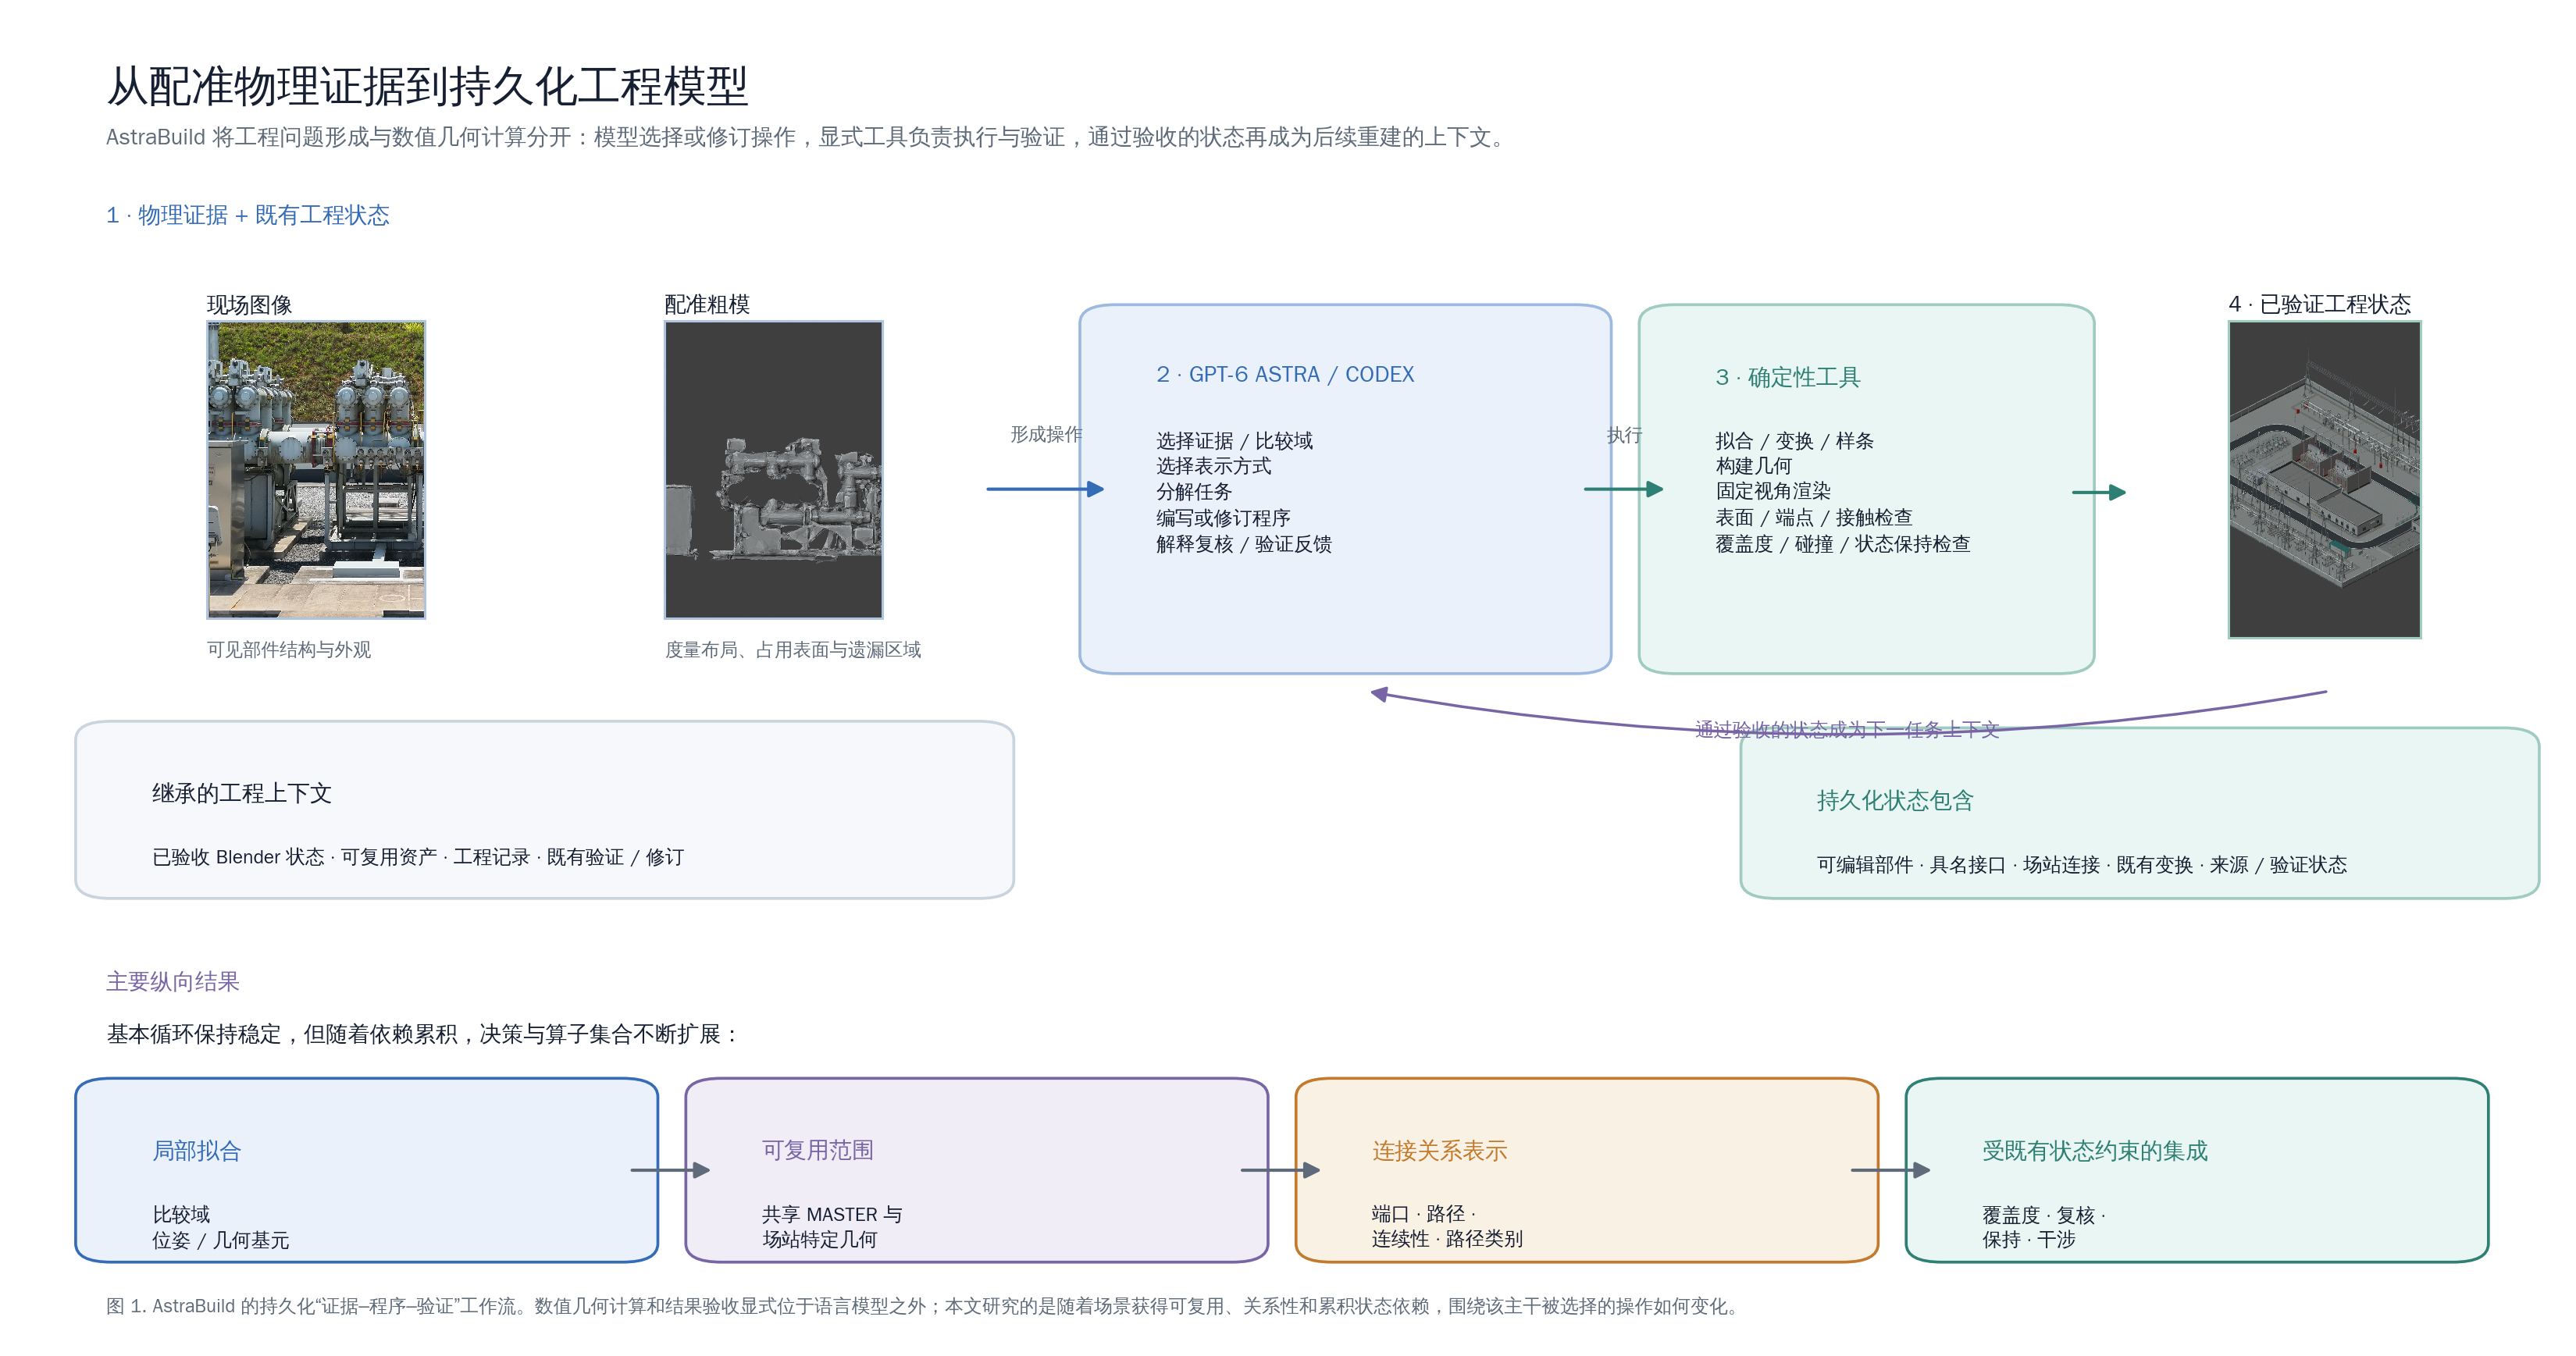
\includegraphics[width=\textwidth,height=0.285\textheight,keepaspectratio]{figures/fig01_problem_method_answer_b01_b36_zh.png}
\caption{AstraBuild 是一个持久化的“证据–程序–验证”工作流。配准物理证据和继承的工程状态共同约束由模型编写或修订的操作；确定性工具执行几何构造和任务特定检查；通过验收的结果进入下一次重建的上下文。图下方概括了本文的纵向结果：共同的工作循环保持稳定，但随着依赖增加，新的表示与集成决策不断出现。}
\label{fig:overview}
\end{figure*}

\hypertarget{ux76f8ux5173ux5de5ux4f5c}{%
\section{相关工作}\label{ux76f8ux5173ux5de5ux4f5c}}

\hypertarget{ux4eceux4e09ux7ef4ux89c2ux6d4bux5230ux7ed3ux6784ux5316ux9006ux5411ux5de5ux7a0b}{%
\subsection{从三维观测到结构化逆向工程}\label{ux4eceux4e09ux7ef4ux89c2ux6d4bux5230ux7ed3ux6784ux5316ux9006ux5411ux5de5ux7a0b}}

AstraBuild 与 CAD
逆向工程研究共享一个目标：将采样几何转化为可编辑、结构化的表示。Point2CAD
通过解析与神经方法相结合的流程，从点云中恢复结构化 CAD 曲面及其拓扑
\citep{liu2024point2cad}。CAD-Recode 则从点云输入预测可执行 Python
代码，以重建参数化 CAD 序列
\citep{rukhovich2024cadrecode}。这些工作都将结构、可编辑性和可执行表示视为重建目标的一部分，而不是把采样表面当作最终结果。

本文场景在尺度和任务结构上有所不同。B01--B36
在同一个继承的变电站场景中，同时涉及设备装配、有限长度的场站连接、柔性导线和土建结构。不同任务需要不同的目标表示，后期几何还受到前序批次中已生成部件和端点的约束。因此，AstraBuild
研究的是一个持久化、异构的逆向工程操作序列，而不是将单个点云映射为某一种固定
CAD 表示的对象级任务。

\hypertarget{ux4f7fux7528ux8bedux8a00ux6a21ux578bux8fdbux884cux7a0bux5e8fux5316ux4e09ux7ef4ux6784ux5efa}{%
\subsection{使用语言模型进行程序化三维构建}\label{ux4f7fux7528ux8bedux8a00ux6a21ux578bux8fdbux884cux7a0bux5e8fux5316ux4e09ux7ef4ux6784ux5efa}}

3D-GPT 与 SceneCraft
直接展示了如何使用语言模型通过可执行程序表达三维构建。3D-GPT
将程序化建模分解为多个协作的语言模型角色，并生成 Blender 操作
\citep{sun2023threegpt}。SceneCraft
构建场景图，将空间关系转化为数值约束与 Blender
代码，渲染场景后再通过视觉反馈进行迭代修订
\citep{hu2024scenecraft}。这些工作表明，语言模型可以操作程序化三维抽象，而不仅仅生成文本描述。

AstraBuild
使用了相似的可执行接口，但推理方向不同。它面对的是一个已经配准的真实物理场站，其几何、部件复用和连接关系受到摄影测量参考、现场图像、工程记录和既有验收状态的共同约束。程序执行后还要接受任务特定的几何验证，通过验收的结果会成为下一次重建问题的一部分。因此，本文关注的不是``语言描述能否合成出合理场景''，而是通用模型如何在物理约束和继承状态下组织不断变化的逆向工程操作。

\hypertarget{ux957fux65f6ux7a0bux5de5ux5177ux4f7fux7528ux667aux80fdux4f53}{%
\subsection{长时程工具使用智能体}\label{ux957fux65f6ux7a0bux5de5ux5177ux4f7fux7528ux667aux80fdux4f53}}

长时程智能体提供了另一类直接相关的概念先例。Voyager
在开放式具身环境中结合可执行代码、环境反馈、迭代程序改进与持久化技能库
\citep{wang2023voyager}。Code as Policies
则将语言模型输出视为可执行程序，并通过程序组合 API 级动作
\citep{liang2023code}。GPT-Policy
研究视觉语言模型如何在约束控制器下工作，并利用示例、演示、反馈和持续运行上下文
\citep{cheng2026gptpolicy}。这些系统提示了一种实验视角：模型的能力应通过其与显式工具和状态的交互来评价，而不是只看一次孤立的文本响应。

AstraBuild
将这一视角应用到真实工业场站的逆向工程。它的动作空间由重建程序和工程算子构成，反馈则包括配准几何、渲染对照、任务特定验证器和继承场景状态。已有工作因此分别提供了三类互补先例：结构化逆向工程、可执行三维生成以及长时程工具使用。B01--B36
则记录了这三类要求如何在同一个持久化工业重建过程中相互作用。

\hypertarget{ux65b9ux6cd5}{%
\section{方法}\label{ux65b9ux6cd5}}

AstraBuild
将部件级场站重建视为一个持续的程序化过程，而不是从图像到几何的一次性推断。该工作流结合通用推理模型、可执行
Blender/Python
程序、配准物理证据、任务特定验证和继承工程状态。模型配置由项目负责人确认，为通过
Codex 使用的 GPT-6 Astra；历史 B01--B36
工件保存了最终产生的程序、计划、诊断图和验证输出，但并未保存模型的私有推理轨迹。因此，本文分析的是可观察到的``模型在执行框架中的行为''及其保存工件。

\hypertarget{ux8bc1ux636eux4e0eux6301ux4e45ux5316ux76eeux6807ux72b6ux6001}{%
\subsection{证据与持久化目标状态}\label{ux8bc1ux636eux4e0eux6301ux4e45ux5316ux76eeux6807ux72b6ux6001}}

每个批次从四类证据中的一个子集出发：配准摄影测量几何、无人机或地面图像、可用时的工程/资产记录，以及从前序批次继承的已验收重建状态。摄影测量参考提供统一空间坐标系和局部表面证据，但本文不将其视为独立测量参考，也不将其视为对物理部件的完整分割。图像用于判断外观、部件结构，以及配准几何缺失或含糊的区域。只有在映射关系有依据时，工程记录才用于提供设备身份或配置信息。

目标不是一个融合表面，而是一个可编辑的部件级 Blender
状态。该状态可以包含可复用部件集合、刚性场站实例、有限长度的场站特定连接、曲线或导线路径、土建几何以及验证/来源记录。通过验收的几何在后续批次中继续可用。历史版本不会被静默覆盖，而是被保留下来，使后续任务既能复用已有部件，也能追溯先前证据和失败状态。

\hypertarget{ux6a21ux578bux4e0eux786eux5b9aux6027ux51e0ux4f55ux5de5ux5177ux7684ux5206ux5de5}{%
\subsection{模型与确定性几何工具的分工}\label{ux6a21ux578bux4e0eux786eux5b9aux6027ux51e0ux4f55ux5de5ux5177ux7684ux5206ux5de5}}

工作流将``问题形成''与``数值几何计算''分离。可观察到的模型侧操作包括：选择相关证据和空间域、选择几何表示、将目标分解为可复用部分和场站特定部分、编写或修订
Blender/Python
程序、选择测量或路径规划算子，以及根据验证或复核输出决定下一步修订。这些操作能够从生成的计划、脚本、修订记录和保存的程序版本中观察到。

数值计算由显式的确定性程序完成。根据任务不同，这些程序包括几何拟合、坐标变换、剖面或样条计算、网格构建、渲染、表面距离计算、端点/接触/连续性检查、碰撞检查以及状态保持测试。验证器会重新打开保存文件并重新计算限定范围内的检查，而不是只依赖构建脚本运行时的内存状态。因此，定量残差描述的是工作流中被选择并执行的显式几何过程的输出，不应被解释为语言模型直接执行高精度数值优化。

\hypertarget{ux6301ux4e45ux5316ux91cdux5efaux5faaux73af}{%
\subsection{持久化重建循环}\label{ux6301ux4e45ux5316ux91cdux5efaux5faaux73af}}

在批次 \(t\) 中，工作流可以概括为

\[
(E_t, S_{t-1}) \rightarrow O_t \rightarrow G_t \rightarrow V_t \rightarrow S_t,
\]

其中，\(E_t\) 表示当前任务选择的证据，\(S_{t-1}\)
表示此前已经验收的工程状态，\(O_t\)
表示通过模型/执行框架形成的可执行重建操作，\(G_t\)
表示最终保存的几何与过程证据，\(V_t\)
表示任务特定验证或复核。验证可能接受当前更新，也可能暴露局部不一致并触发修订操作。被接受的结果成为
\(S_t\)
的一部分，后续批次可以通过命名集合、变换、端口和端点直接寻址这些结果。

验证标准取决于所表示的几何类型。局部刚性结构可以使用限定区域内的表面对照；连接系统还要求端点与接触约束；遗漏发现使用选定区域的覆盖度；后期批次还检查继承变换是否保持，并在必要时检查几何干涉。这种异构性是有意保留的：本文不使用一个统一残差来表示整站精度。

\hypertarget{b23-ux793aux4f8bux6539ux53d8ux8868ux793aux800cux4e0dux662fux7ee7ux7eedux8c03ux53c2}{%
\subsection{B23
示例：改变表示而不是继续调参}\label{b23-ux793aux4f8bux6539ux53d8ux8868ux793aux800cux4e0dux662fux7ee7ux7eedux8c03ux53c2}}

B23
清楚展示了``表示选择''和``数值拟合''之间的分工。继承的预检方案主要把一条主变中性点连接视为两端点之间的直线问题。对配准参考的检查表明，轨迹中部存在约
0.5 m
的横向弯曲，说明直线表示漏掉了可见的源几何。于是，重建操作被重新表述为受约束的曲线路径：源几何按空间分箱，提取
8 个控制点，再由确定性代码拟合端点固定、带平滑惩罚项的三次 B
样条。保存后的路径终止于已有 B08
主变端子接口，并通过有限源域和端点检查进行评价。

第一次修订后的几何仍不能解释附近全部结构。B23
的后续修订增加了柔性连接和下部桥接接触，同时保持此前状态与固定比较域不变。从方法角度看，关键在于决策顺序：工作流首先把几何假设从直线段改为曲线路径，随后数值拟合在该表示中估计参数，最后验证保存结果并可能触发下一轮局部修订。B01--B36
的其他任务中也存在同类模式，只是使用了不同算子，例如 B15
中可复用范围的修订，以及 B20 与 B36 中的路径/干涉修订。

\hypertarget{ux7814ux7a76ux8bbeux8ba1}{%
\section{研究设计}\label{ux7814ux7a76ux8bbeux8ba1}}

\hypertarget{ux8fdeux7eedux91cdux5efaux8bb0ux5f55}{%
\subsection{连续重建记录}\label{ux8fdeux7eedux91cdux5efaux8bb0ux5f55}}

本文把 B01--B36 作为一条来自实际运行 220 kV
变电站的连续重建记录来分析。后续批次继承前序批次已经验收的几何、可复用资产、变换和验证状态。重建目标也随时间变化：早期工作集中在局部设备与土建拟合，中期开始出现重复设备族和显式连接，而最后几批则在已经很大的累积场景中处理剩余土建与辅助设施。由于几何类型、依赖结构和任务特定验证在不同批次间并不相同，本文不会把
36
个批次压缩成一个统一成功率，而是分析随着依赖增加，重建操作本身如何变化。

为便于理解，图 2
将时间轴划分为四个描述性区段：局部拟合结构（B01--B06）、重复设备（B07--B19）、连接系统（B20--B30）和场站闭合（B31--B36）。这些区段仅用于概括目标结构，并不被视为从数据中发现的正式任务阶段，也不构成统一难度尺度。结果部分按照代表性案例能够支持的科学主张来组织，而不是逐区段展开。

\hypertarget{ux5206ux6790ux4f7fux7528ux7684ux8bc1ux636e}{%
\subsection{分析使用的证据}\label{ux5206ux6790ux4f7fux7528ux7684ux8bc1ux636e}}

保留的历史记录包含多种工程证据。固定相机下的 Clean、Overlay 和 Reference
渲染允许在视角不变的条件下比较模型与配准源。对于可以定义有限比较域的对象，局部表面检查用于量化限定范围内的几何一致性。连接系统验证器还会增加端点、接触和连续性检查，这些条件不能被简单归约为表面距离。B25/B26
引入了选定区域覆盖度诊断，用于寻找大型未解释结构；后期批次则记录既有对象、变换、集合和受保护文件是否保持。这些证据回答的是不同问题，因此本文始终按照其局部适用范围报告，而不把它们合并为一个整站精度指标。

§5.1 中的算子分析来自保存的阶段/脚本工件和复核记录。在 B01--B36
的目录中，\texttt{build} 与 \texttt{validate} 出现在全部 36
个批次中，而其他命名阶段随目标而变化。本文仅将这一记录作为纵向分析的描述性导向。某个命名阶段没有出现，并不意味着不存在推理，也不被视为性能失败。§5.2
中对机制的解释则主要依赖直接工件，例如测量域、可复用 MASTER
边界、端口清单、路径规划、剖面拟合、覆盖度诊断以及碰撞/干涉修订记录。

主文不会对 36 个批次给予相同叙事权重。B01/B02 建立局部测量问题；B08 与
B15 揭示可复用几何与场站特定几何之间的边界；B20、B23 和 B29
提供连接系统证据；B25/B26 将未解释几何覆盖度作为额外的任务选择信号；B36
则提供序列末期最清楚的组合与干涉案例。B06、B17/B19、B31/B32 和 B35
用作补充性的视觉或结构证据。完整批次历史、原始 review
页面、修订文件与任务局部指标记录更适合放在补充材料或网站证据浏览器中。

\begin{figure*}[!t]
\centering
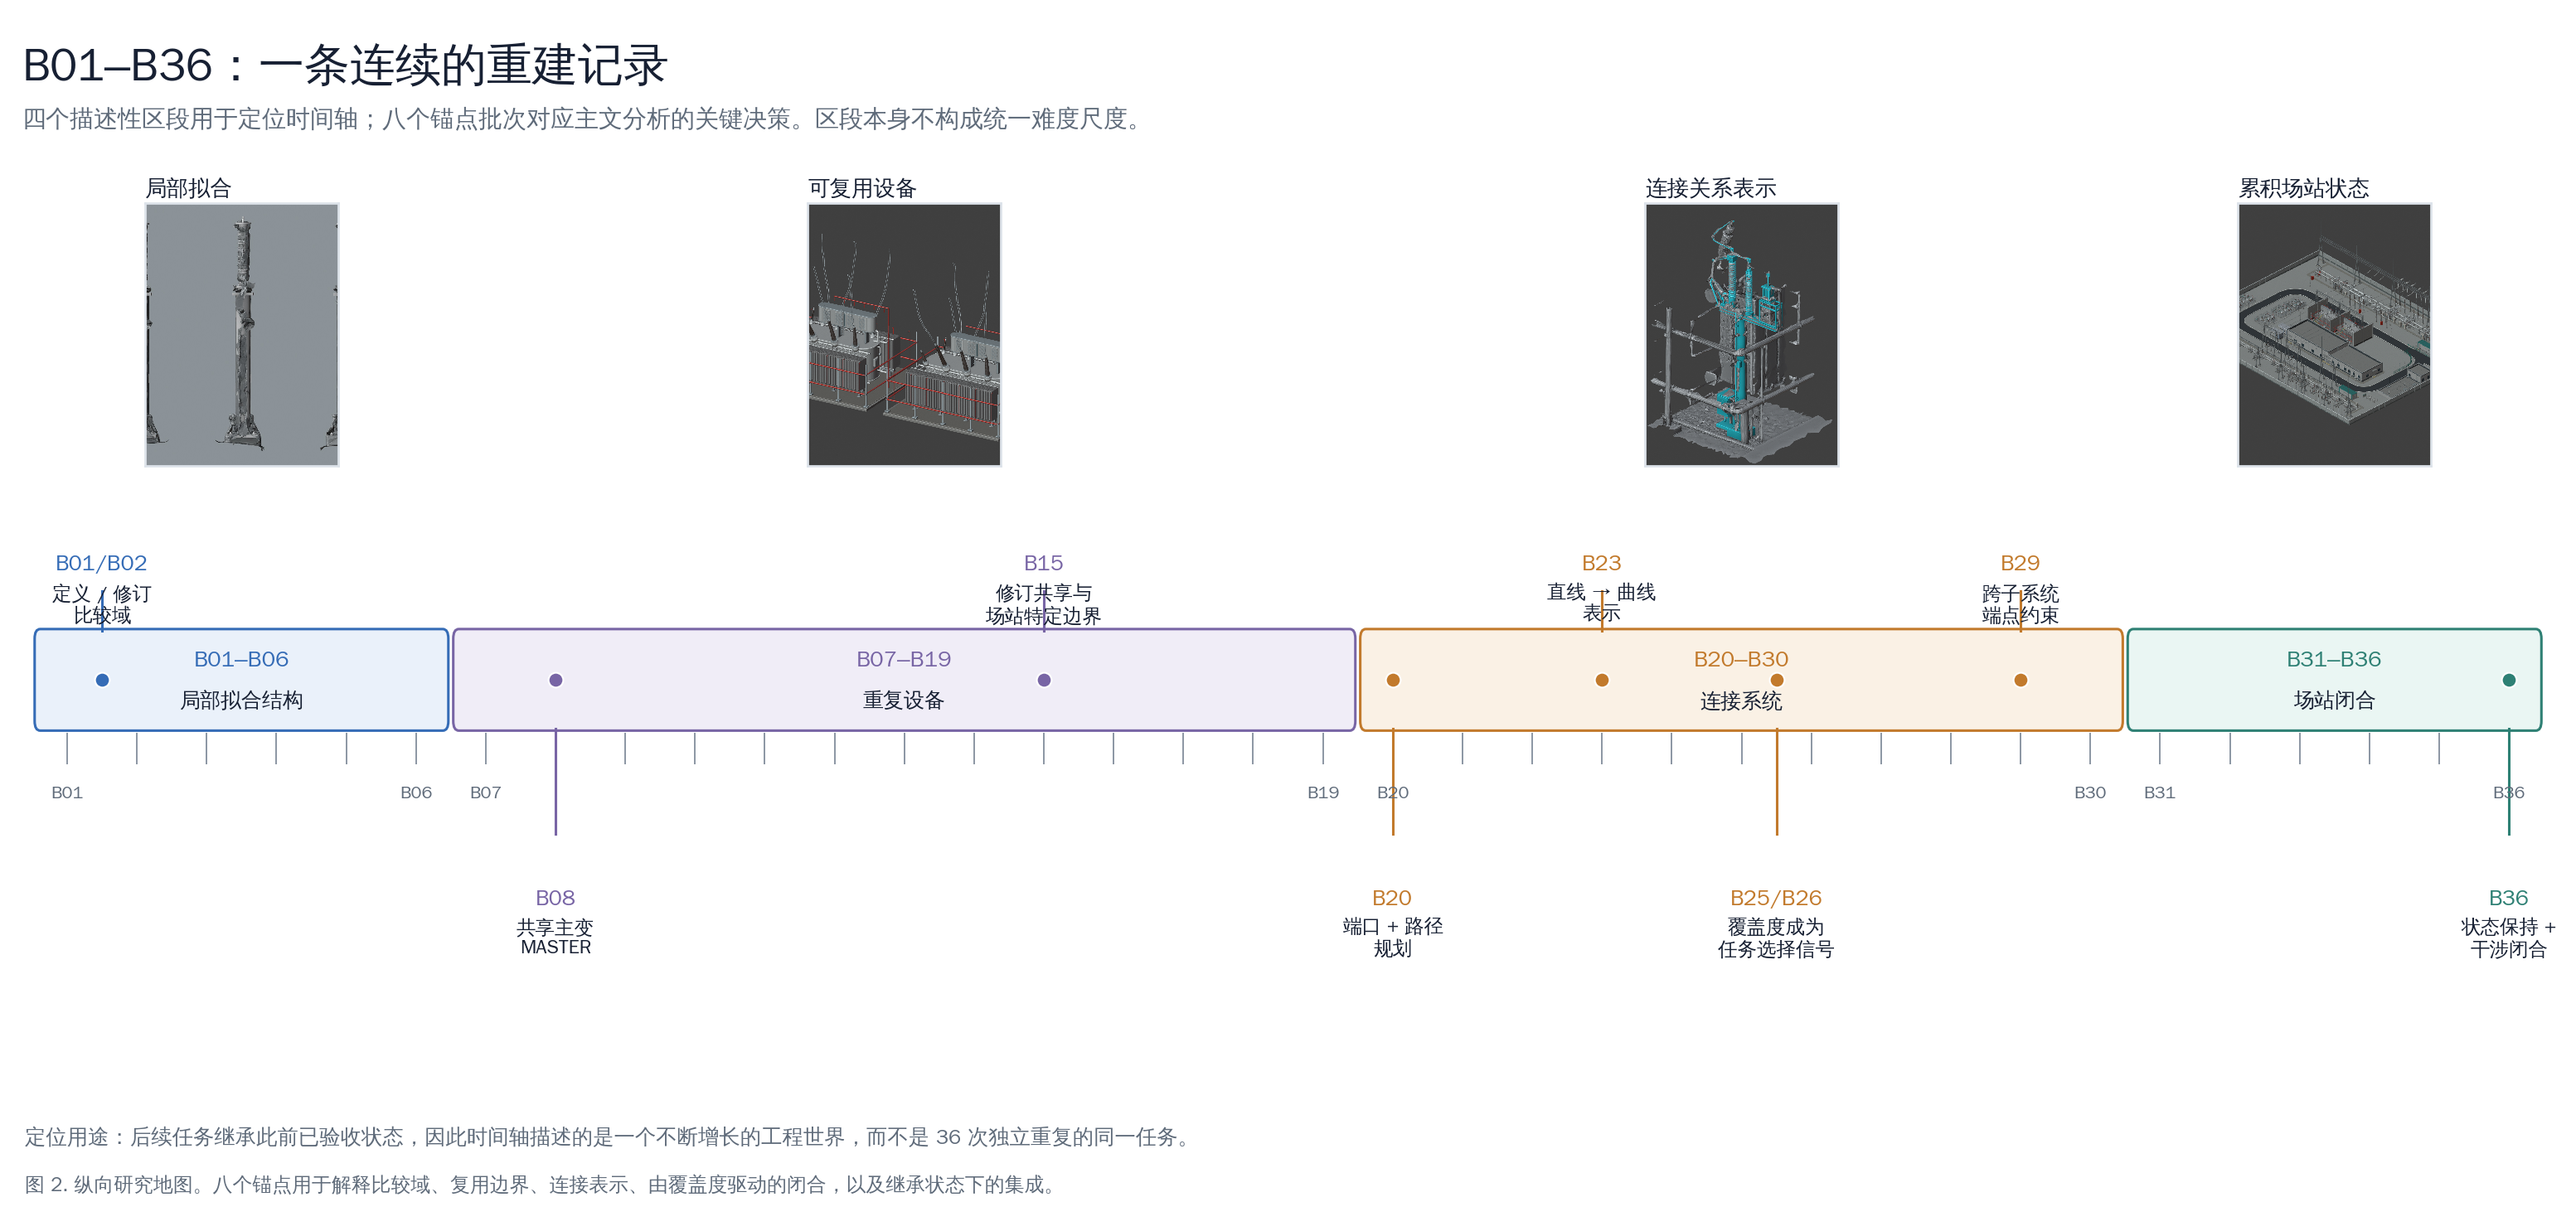
\includegraphics[width=\textwidth,height=0.255\textheight,keepaspectratio]{figures/fig02_longitudinal_map_b01_b36_zh.png}
\caption{纵向研究地图。四个描述性区段用于帮助读者定位不同重建目标，但不定义统一难度尺度。八个锚点批次对应主文中用于分析的关键证据：比较域、复用边界、端口与路径、表示改变、由覆盖度驱动的闭合、端点组合以及受干涉约束的后期集成。}
\label{fig:timeline}
\end{figure*}

\hypertarget{ux7ed3ux679c}{%
\section{结果}\label{ux7ed3ux679c}}

结果部分分析 B01--B36
记录中的两个核心性质。首先，我们考察随着被重建对象获得更多依赖关系，算子集合如何变化，并通过三个结构性转变解释这些变化。随后，我们分析局部解决方案是否确实通过持久化外部工程状态被组合起来，以及这种机制所带来的错误传播风险。

\hypertarget{ux91cdux5efaux5faaux73afux4eceux5c40ux90e8ux62dfux5408ux6269ux5c55ux4e3aux66f4ux5e7fux7684ux7b97ux5b50ux7ec4ux5408}{%
\subsection{重建循环从局部拟合扩展为更广的算子组合}\label{ux91cdux5efaux5faaux73afux4eceux5c40ux90e8ux62dfux5408ux6269ux5c55ux4e3aux66f4ux5e7fux7684ux7b97ux5b50ux7ec4ux5408}}

从 B01 到
B36，始终可以辨认出相同的基本重建循环：提取或检查配准证据，形成可执行几何操作，构建结果，并对保存状态进行验证。发生变化的是围绕这一主干所需的算子集合。最早的记录主要由直接拟合构成；后期任务仍保留局部测量，但逐步加入规划、细化、复核、连接关系、覆盖度和干涉处理。这一模式是描述性的，而非统计规律：它来自保存的脚本、计划、诊断图和
review 工件，某个命名阶段未出现并不意味着没有推理或任务失败。

这种差异在序列开端最为明显。B01--B06 的每个批次都记录了显式 \texttt{fit}
阶段，而保存目录中没有独立的
\texttt{measure}、\texttt{plan}、\texttt{refine} 或 \texttt{audit}
阶段。这些任务大体可以表述为局部几何问题：选择相关源区域，估计刚体位姿或简单几何基元，再与配准参考比较。B01/B02
表明，即使是这种相对简单的情况，也需要正确界定比较域；但一旦比较域确定，计算结构仍然很紧凑。

当重复设备和连接系统成为主要目标后，算子记录显著变宽。B07--B19 的 13
个记录中，\texttt{measure} 出现 8 次、\texttt{plan} 7
次、\texttt{refine} 9 次、\texttt{audit} 10 次，并且 13
个批次全部保存了交互式 review 页面。B20--B30 的 11 个批次中，显式
\texttt{inspect} 与 \texttt{plan} 各出现 8 次，\texttt{audit} 出现 10
次，同时出现了早期局部拟合阶段没有的路径、特征和覆盖度工件。局部拟合仍然存在：这
11 个批次中有 6 个仍包含显式
\texttt{fit}，但它已经嵌入一个更大的关系性操作集合中。

B31--B36
也体现出同样的累积，而不是从几何问题``干净地切换''到另一类任务。6
个批次全部包含显式测量，5 个包含检查，4 个包含规划，5 个包含专门 review
阶段；B36
还新增了显式碰撞/干涉操作。这些记录对应的是这样一种场景：后期任务必须解释不完整的源几何，保持一个大型继承模型，并在已有设备和连接周围插入新结构。图
3 汇总了全部 36
个批次的算子集合；下一节再通过直接的计划、剖面和验证记录解释为什么会出现这些新增决策层。

\begin{figure*}[!t]
\centering
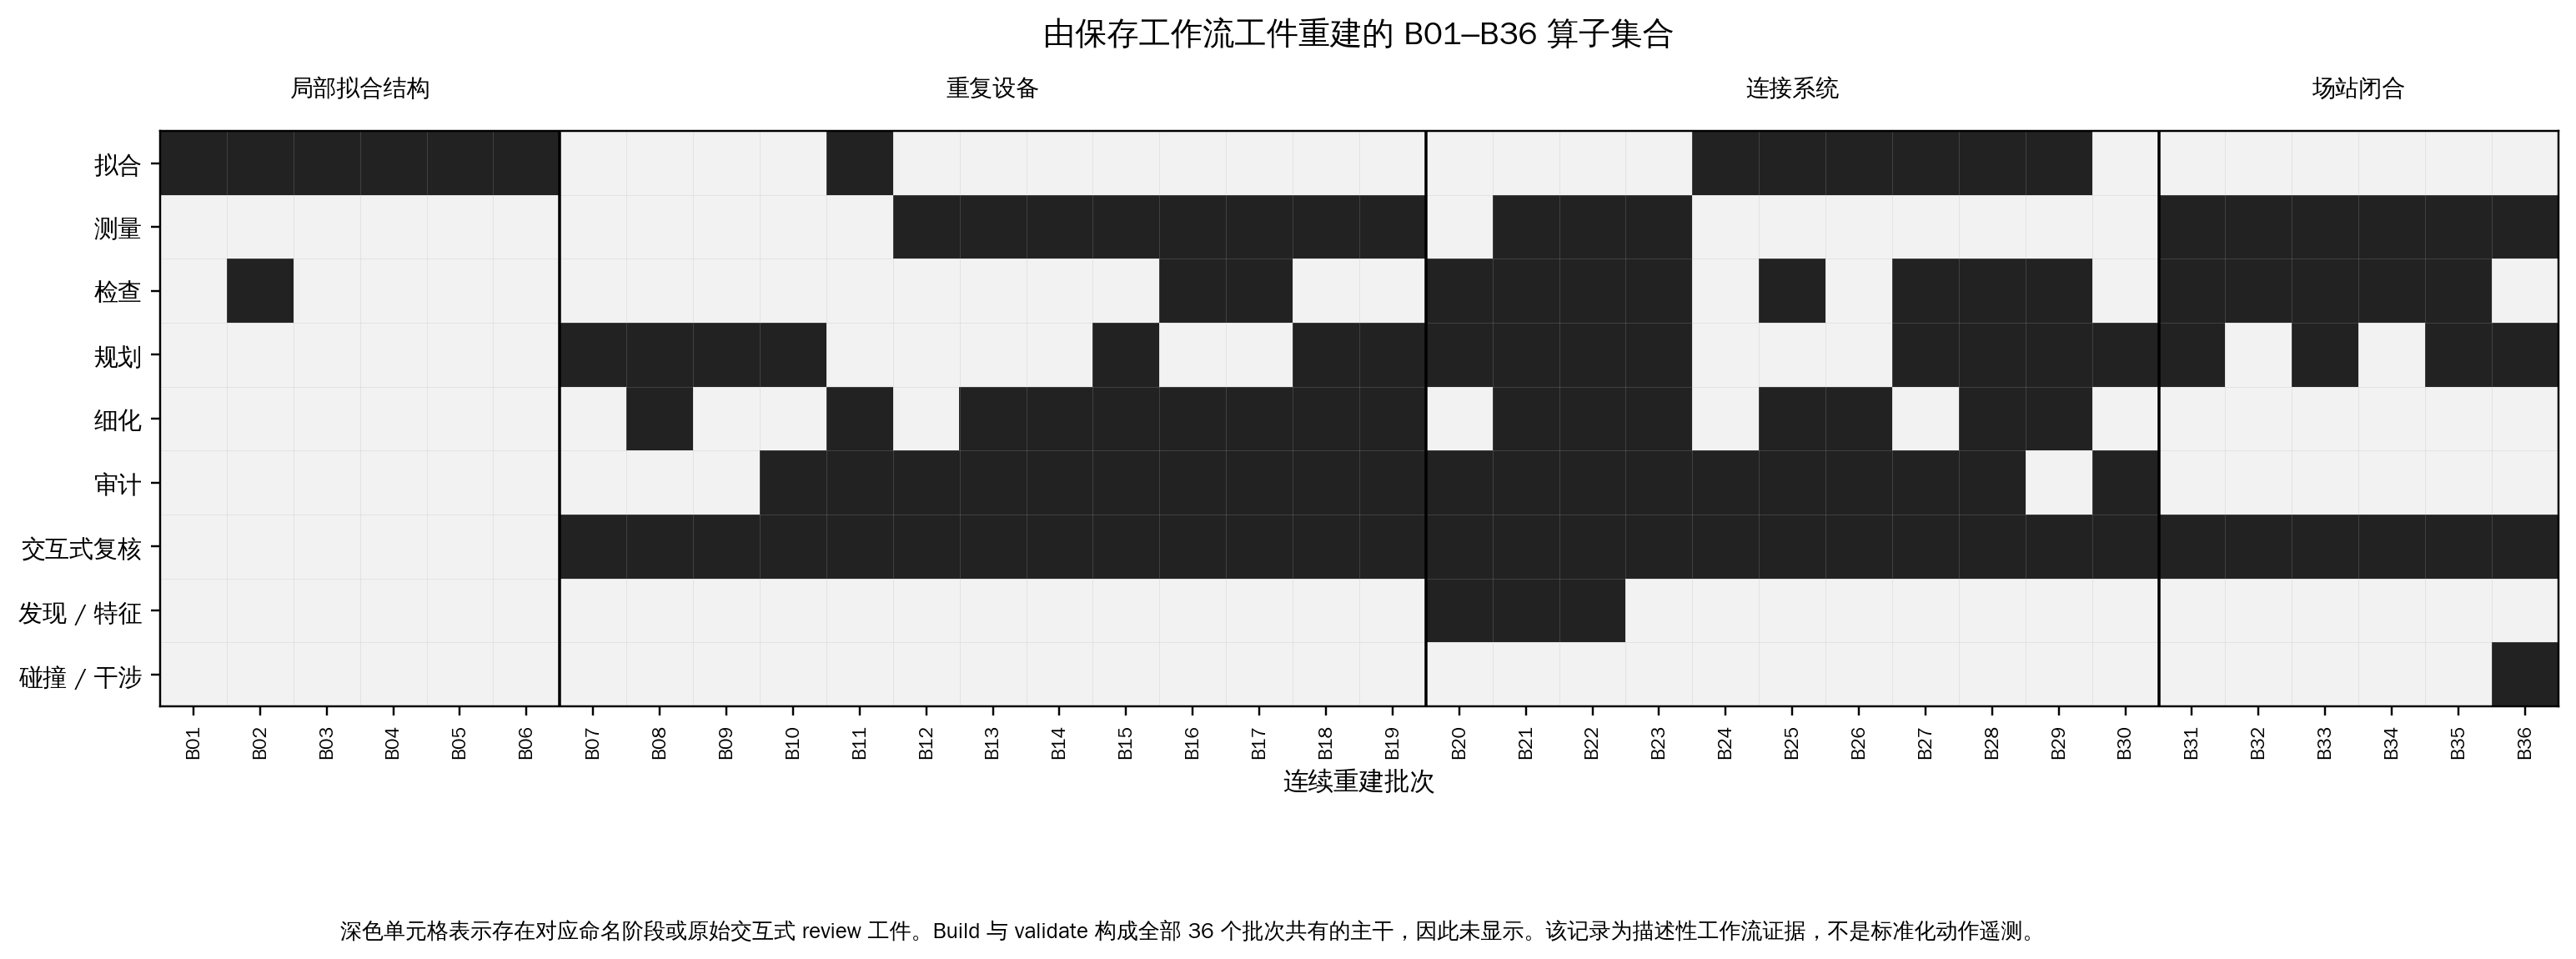
\includegraphics[width=\textwidth,height=0.245\textheight,keepaspectratio]{figures/fig03_operator_portfolio_b01_b36_zh.png}
\caption{根据保存的阶段脚本和原始 review 工件重建的描述性算子集合。Build 与 validate 构成全部批次共有的主干，因此未在矩阵中显示。深色单元格表示存在对应命名阶段或原始交互式 review 工件；空白单元格不被解释为失败，也不意味着不存在推理。}
\label{fig:operators}
\end{figure*}

\hypertarget{ux4e09ux4e2aux7ed3ux6784ux6027ux8f6cux53d8ux89e3ux91caux4e86ux4e3aux4ec0ux4e48ux91cdux5efaux5faaux73afux9700ux8981ux6269ux5c55}{%
\subsection{三个结构性转变解释了为什么重建循环需要扩展}\label{ux4e09ux4e2aux7ed3ux6784ux6027ux8f6cux53d8ux89e3ux91caux4e86ux4e3aux4ec0ux4e48ux91cdux5efaux5faaux73afux9700ux8981ux6269ux5c55}}

B01--B36
始终保留``证据选择---可执行几何---验证''这一可识别结构，但随着对象之间开始形成依赖，围绕这一循环所需的工程决策发生变化。这种变化并不是低层几何拟合被一种全新的过程替代；后期批次依然持续使用局部测量与拟合。真正新增的是围绕局部几何的决策层：重复设备要求显式确定可复用结构与场站特定结构之间的边界；连接系统要求端口、路径、连续性与表示选择；场站后期工作则要求识别剩余缺口，并把新几何插入已经高度填充的场景中。下面的三个转变均由保存的批次工件支撑，而不是把时间顺序本身当作任务难度。

\hypertarget{ux4eceux51e0ux4f55ux62dfux5408ux5230ux5b9aux4e49ux53efux590dux7528ux8303ux56f4}{%
\subsubsection{从几何拟合到定义可复用范围}\label{ux4eceux51e0ux4f55ux62dfux5408ux5230ux5b9aux4e49ux53efux590dux7528ux8303ux56f4}}

最早的批次展示了最简化的重建问题：先定义需要比较的局部几何，再求解显式几何参数。B01
使用一个冻结的源资产放置三个避雷器候选，共享尺度，并为每个实例估计刚体位姿。验证有意保留了未通过
5 cm
内部筛查的结果：宽泛的圆柱比较区域包含突出的附件和不规则粗模表面，因此三个候选的
RMS 分别为 4.84、7.32 和 5.10 cm。B02
并不是在同一目标函数上做更强的优化，而是重新定义拟合与验证区域，使其只包含裸露柱体表面，同时保持制造源几何不变；历史记录还明确指出，两轮评价不能直接比较。因此，工程决策的一部分本身就是``测量问题如何定义''。一旦比较域确定，数值拟合与残差计算仍由确定性代码执行。

重复设备带来了不同的问题。B08 在用户明确确认 T1 与 T2
使用相同部件配置后，通过一个共享的 \texttt{B08\_TRANSFORMER\_MASTER}
和两个刚性场站根节点表示两台主变。外部导线线路径不属于共享
MASTER，而是分别针对两个安装位置追踪。保存的验证器检查共享
MASTER、两个刚性根节点，以及一次共享修改是否能传播到两个实例。这个表示并不仅仅是一种方便的对象层级；它显式表达了哪些几何被假设为跨安装位置不变，哪些几何允许随场站上下文变化。

B15
表明这一边界具有直接物理意义。一个较早版本把相同的有限母线短管范围分配给多个
GIS
安装实例，导致实际相邻间距不同的位置出现重叠。修订因此改变了表示边界：公共设备几何继续保持可复用，而有限长度的管段和支撑被移到场站特定包装层，并按照真实邻近端点重新构建。对于
752--502 和 754--501
等距离很近的设备对，通过裁剪重叠附加段处理；其他设备对则由在计算中点处相接的有限段连接。最终验证对这些建模接口报告了亚毫米级数值端点闭合，同时保留了若干尚未解决的局部表面检查。因此，关键结论并不是``复用始终成功''，而是：一旦出现重复设备，复用边界本身就成为重建变量，工作流必须判断哪些几何属于共享设备描述，哪些几何只属于某个具体安装位置。

\hypertarget{ux4eceux5bf9ux8c61ux51e0ux4f55ux5230ux8fdeux63a5ux5173ux7cfbux8868ux793a}{%
\subsubsection{从对象几何到连接关系表示}\label{ux4eceux5bf9ux8c61ux51e0ux4f55ux5230ux8fdeux63a5ux5173ux7cfbux8868ux793a}}

当被重建部件必须彼此发生关系时，局部表面对齐已经不足以定义完整问题。B20
通过直接读取此前已建设备的真实末端建立端口清单，并利用这些端口规划 21
个相邻区间，从而清楚地体现了这一转变。规划文件区分已连接接口、新的直线段，以及
4100
区域中无法通过沿排布方向简单直连来表示的一条剩余路径。记录还明确区分几何连接关系与电气身份。此时，一个连接不再被视为``放在粗模附近的独立物体''，而被表示为已有端点之间的关系与一条路径。

B23
更直接地展示了表示选择。继承的预检主要把主变中性点连接视为两端点之间的直线路径。对配准源的检查显示，轨迹中部约有
0.5 m
的横向弯曲。因此重建操作被重新表述：源几何被分箱、控制点被提取，然后由确定性代码拟合端点固定、带平滑惩罚项的三次
B
样条。随后几次修订又增加了柔性连接和桥接接触，因为第一版修订表示仍未解释所有可见结构。真正重要的改变发生在样条系数计算之前。直线段与受约束曲线路径代表两种不同的几何假设，在错误的表示类别中继续降低残差并不会恢复缺失的中部弯曲。

B29
则把同类关系扩展到更大的系统尺度。该批次新增耐张串、跳线和跨场导线，它们的端点直接绑定到此前已建的线夹、悬垂端以及由变压器引线派生的端点。验证器分别检查保存后的导线端点、已有接口和粗模表面一致性。这个区分非常重要：某些局部源域因为同时包含分支、线夹或尚未建模的结构，会产生较大的表面残差，但预期端点关系仍可满足数值容差。对连接系统而言，拓扑与端点一致性因此构成一种不同于局部表面拟合的工程标准。重建问题也从``估计一个对象的形状''扩展为``选择一种能满足已建对象之间显式关系的表示''。

\hypertarget{ux4eceux9884ux5b9aux76eeux6807ux6dfbux52a0ux5230ux7531ux7f3aux53e3ux4e0eux65e2ux6709ux72b6ux6001ux9a71ux52a8ux7684ux95edux5408}{%
\subsubsection{从预定目标添加到由缺口与既有状态驱动的闭合}\label{ux4eceux9884ux5b9aux76eeux6807ux6dfbux52a0ux5230ux7531ux7f3aux53e3ux4e0eux65e2ux6709ux72b6ux6001ux9a71ux52a8ux7684ux95edux5408}}

随着主要设备和连接逐渐累积，下一个重建目标已经不能只依赖资产清单可靠地选择。B25
将配准高位区域几何与当前模型场景进行比较，发现 GIS
与主变区域上方仍存在距离较大的高位结构，这些结构尚未被现有模型解释。由此暴露出的缺口触发了后续重建。在选定区域中，GIS110
的中位距离在构架工作后从 1.75 m 变为 0.10 m，GIS220 的中位距离从 8.12 m
变为 0.15 m。B26
将同样逻辑应用于主变/防火墙区域；其选定高位区域中位距离从 3.15 m 变为
0.06 m，距离模型超过 1 m 的选定样本比例从 78.8\% 变为
14.6\%。这些数值是对同一个配准重建中选定区域的诊断，并不是独立的整站完整性度量。它们在工作流中的作用更窄也更具体：未解释几何成为决定``下一步该建什么''的额外信号。

随后进行的土建和辅助设施批次仍包含显式测量，但它们已经工作在一个不同的上下文中。B31
在包含数万对象的场景中拟合主建筑，同时保持七千多个既有场站变换不变。缺失或不完整的屋顶表面不是被当作直接测量几何，而是结合现场图像与相对结构证据补充。B32
同样把拟合得到的舱体包络与可复用端墙/HVAC
和门部件结合起来，并在照片和源几何台阶证据与继承假设冲突后修正门的位置解释。到
B35，保存记录已经明确限定交付物只覆盖可见室外模型，不包含隐藏、地下和不确定结构。因此，当配准源不完整或含糊时，固定相机复核成为局部数值拟合的重要补充。

B36
是后期最清楚的例子，因为新几何同时受到源证据、继承端点和已有空间占用的约束。该批次补建剩余主变侧母线构架，同时保持共享
B08 主变装配不变。6 条新的主母线路径终止于已有主变 stub
和新的墙套管，验证器在保存模型中检查这些端点关系。修订历史还保留了一次非有限数值失败草稿、后续的截面方向修正，以及最终为避开已有消防立管而进行的最大
0.16 m
局部位移，同时保持预定端点和支撑位置。到了这一阶段，任务已经不能再准确描述为``把一个目标拟合到一个参考裁剪''。一个有效更新必须既解释新的源几何，又与一个已经包含可复用资产、连接点和物理占用的工程世界兼容。

综合来看，这三个转变描述的是决策与算子集合不断扩展，而不是低层几何被``更高层''推理单调替代。B01/B02
主要围绕比较域定义；B08/B15
增加共享结构与场站特定结构的边界；B20/B23/B29
增加端口、路径、连续性和表示类别；B25/B26 到 B36
又进一步加入遗漏发现、复核、既有状态保持和干涉约束。这是对一个历史重建序列的描述性结果，不是普适的复杂度规律，也不能证明模型随着时间学会了更复杂的技能。但它解释了为什么
B01--B36
不能被还原为反复执行同一个拟合基元。下一节讨论使这些后期依赖真正可实现的机制：跨批次复用的持久化外部工程状态，以及当上游抽象错误时，同一状态如何传播错误。

\begin{figure*}[!t]
\centering
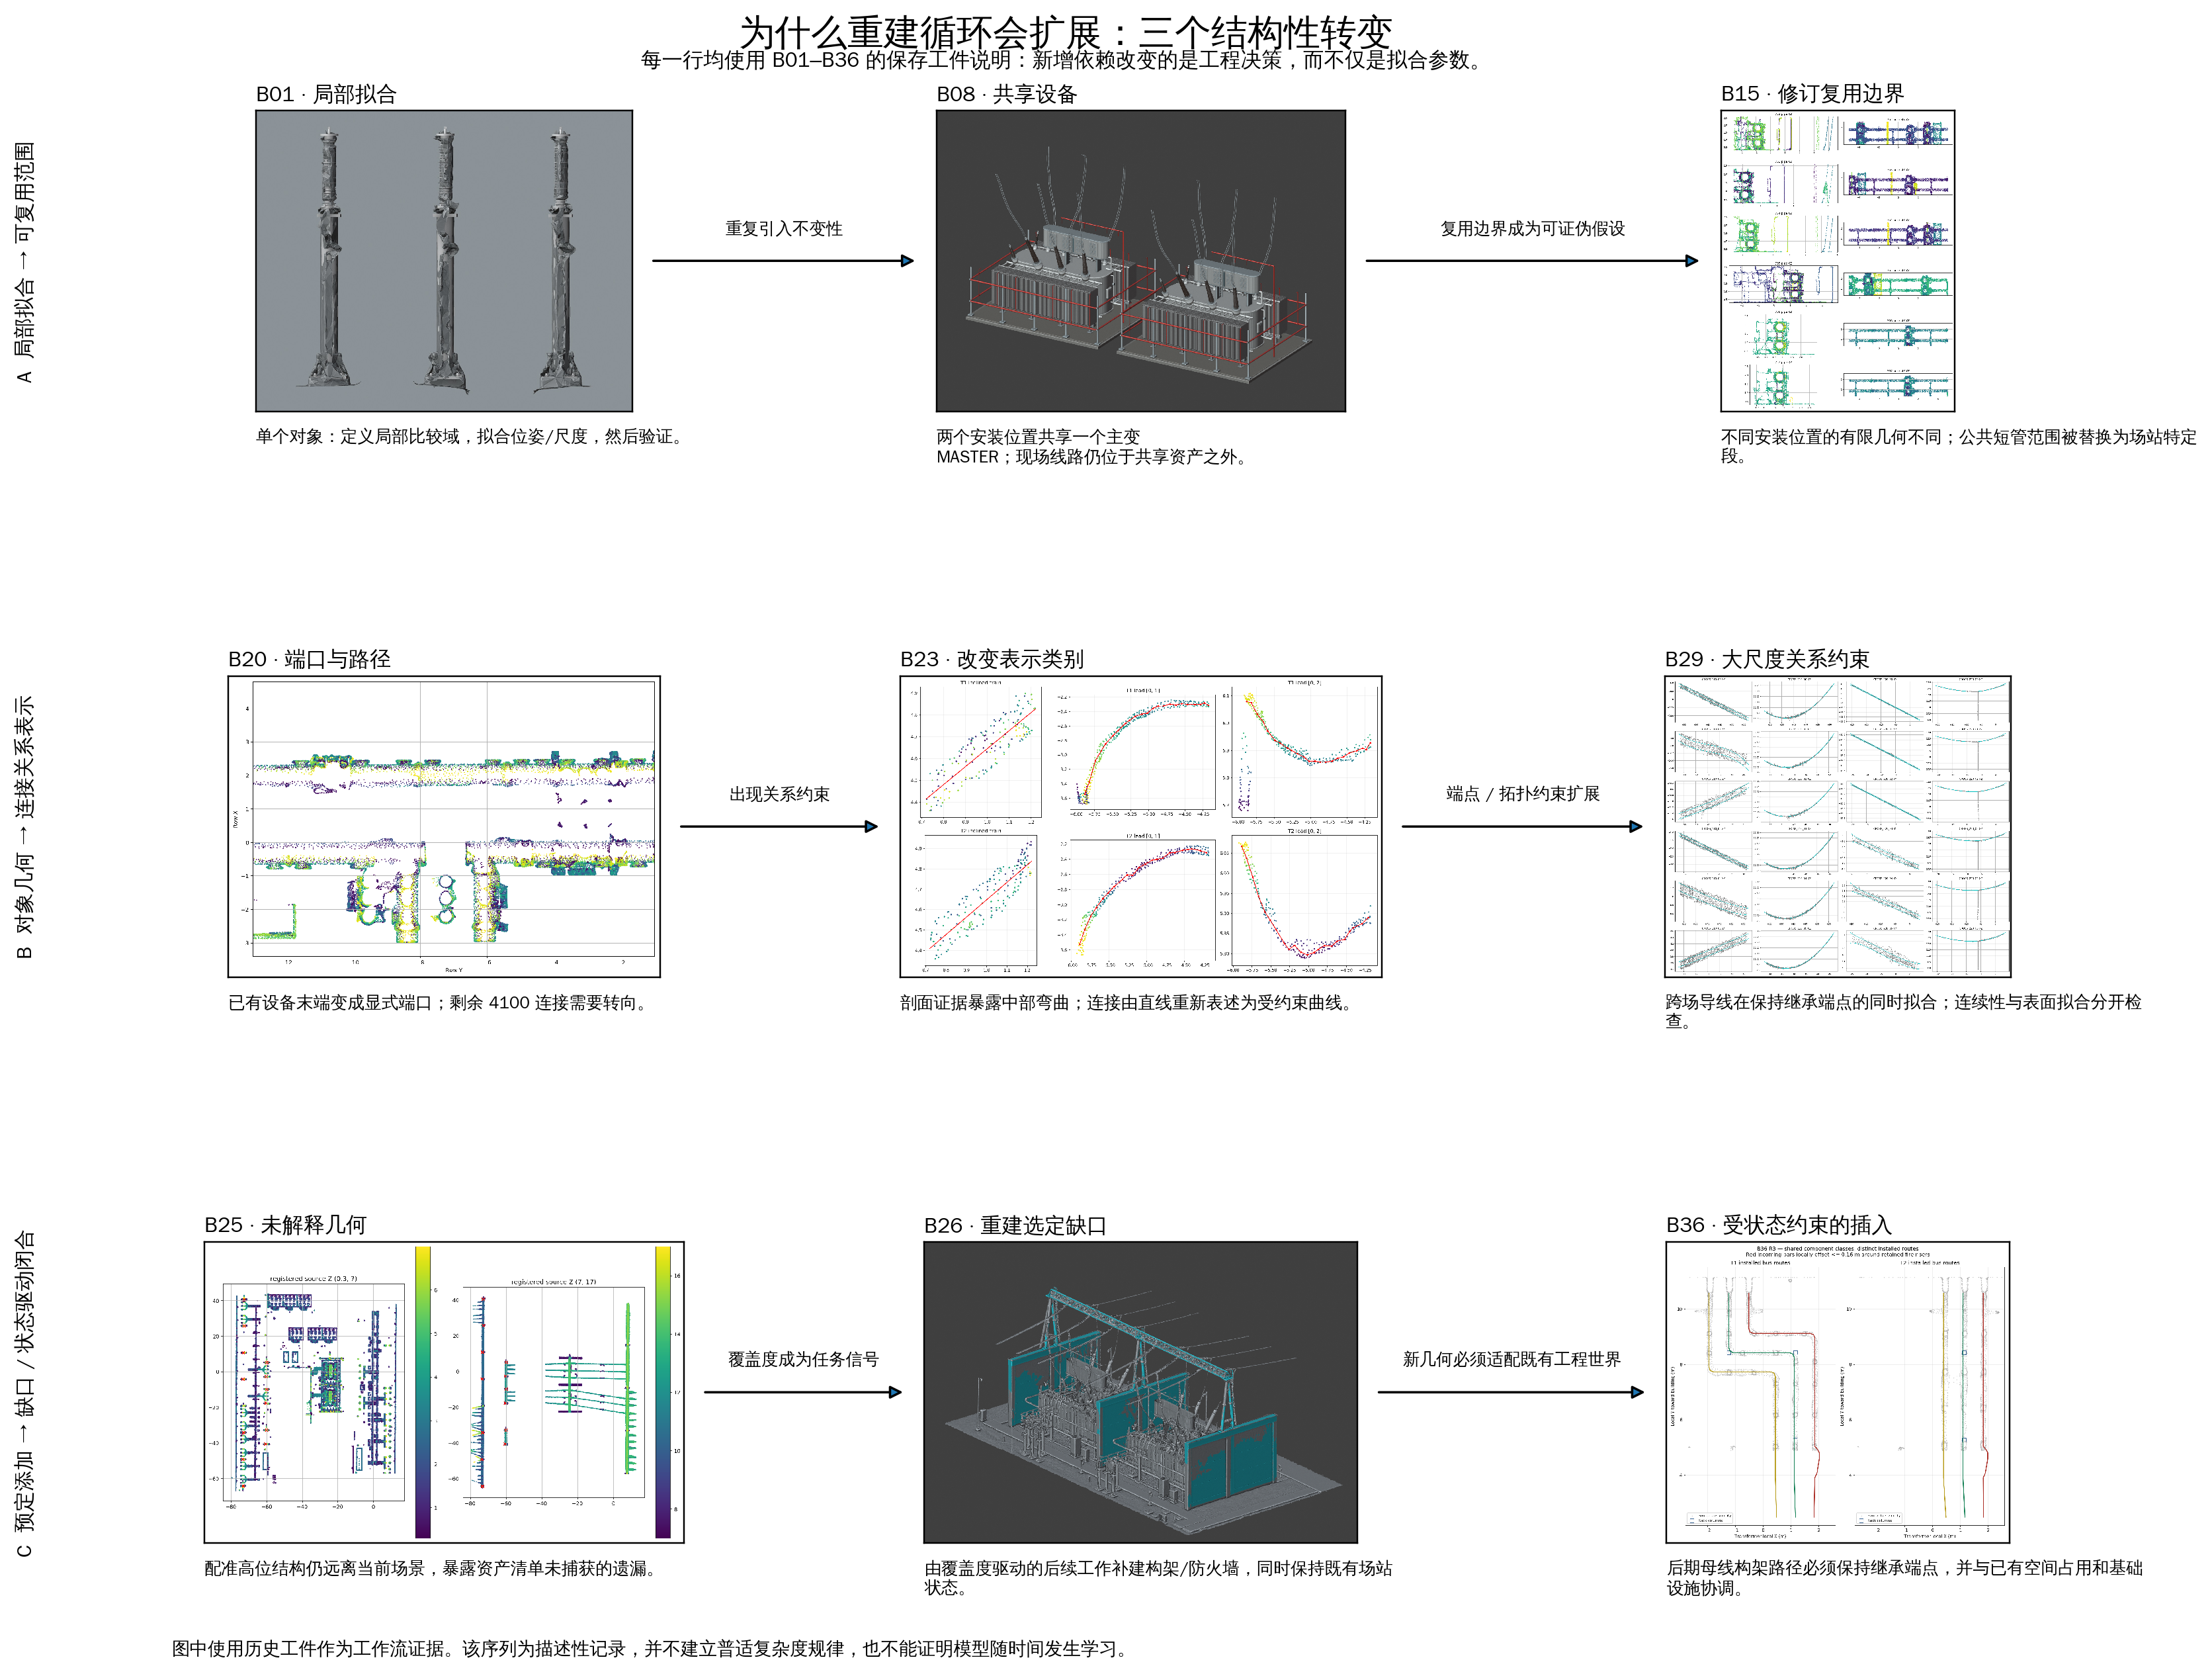
\includegraphics[width=\textwidth,height=0.335\textheight,keepaspectratio]{figures/fig04_structural_transitions_b01_b36_zh.png}
\caption{三个由保存历史工件支撑的结构性转变。重复设备引入可复用/场站特定边界；连接系统引入显式端口、路径与表示选择；后期闭合利用未解释几何与继承空间占用来选择并约束新工作。图中案例来自 B01–B36，用于描述工作流变化，而不是定义普适复杂度分类。}
\label{fig:transitions}
\end{figure*}

\hypertarget{ux6301ux4e45ux5316ux5916ux90e8ux72b6ux6001ux4f7fux5c40ux90e8ux89e3ux80fdux591fux7ec4ux5408ux4e5fux4f1aux4f20ux64adux62bdux8c61ux9519ux8bef}{%
\subsection{持久化外部状态使局部解能够组合，也会传播抽象错误}\label{ux6301ux4e45ux5316ux5916ux90e8ux72b6ux6001ux4f7fux5c40ux90e8ux89e3ux80fdux591fux7ec4ux5408ux4e5fux4f1aux4f20ux64adux62bdux8c61ux9519ux8bef}}

B01--B36 后期批次并不是一组恰好共存在同一个 Blender
文件中的独立重建。它们会显式使用前序批次生成的几何、变换、端子和可复用部件，而验证脚本则检查继承状态是否保持不变。因此，AstraBuild
的长时程性是通过一个持久化外部工程状态实现的：此前已经验收的几何会成为后续重建问题本身的一部分。这一机制支持跨批次组合，但也使共享表示中的错误变得具有后果，因为这些假设会被后续工作继承。

B08
建立了一个清晰的可复用状态对象。在明确确认两台主变拥有相同部件配置后，该批次通过一个
\texttt{B08\_TRANSFORMER\_MASTER}
与两个刚性场站根节点表示两台设备。场站特定导线路径不进入
MASTER。验证器检查 MASTER
是否共享、场站根节点是否保持刚性，以及共享修改是否能传播到两个实例。这样的组织使后续批次能够寻址稳定的几何与接口。其意义并不在于主变装配中包含多少网格，而在于部件几何和端子位置成为持久化、具名的场景组成部分。

B23 直接使用了这一先前状态。其新建中性点引线终止于已有 B08
主变端子端口，而不是重新估计一个替代端点。该批次在增加新的共享机构和场站特定连接时，保持继承的
B08
装配及数千个历史世界变换不变。因此，这条连接是相对于工程模型中已经存在的接口来定义的。这构成了一个直接的跨批次依赖：下游任务把先前建模得到的端子作为自身边界条件的一部分。

B29
将相同模式扩展到多个子系统。新的耐张串、跳线和跨场导线连接到此前建模的线夹、悬垂端以及由主变引线派生的端点。保存后的验证分别检查端点连续性和源表面一致性，同时保持先前场站状态。此外，后续下引线的规划工件直接从已保存几何中派生端子坐标，而不是重新从粗模估计这些设备。由此，工作场景逐步积累出一组可以被后续操作直接寻址的接口。

B36
是这条依赖链最清楚的终点。该批次新增主变到建筑侧的母线构架装配，同时保持
B08 主变装配不变。6 条新的主母线路径终止于已有主变 stub
和新的墙套管，验证器在保存模型中检查这些连接。同时，它记录了 36,615
个既有对象、7,114 个既有场站变换和 2,798
个受保护文件保持不变；最终文件包含 36,812 个对象和 7,116
个场站对象。这些数值描述的是状态规模与保持负担，并不是经独立核验的真实物理资产数量。关键观察在于：新的更新必须与许多批次之前创建的具体接口保持兼容，同时不能破坏已经积累的工程世界。

持久化也会带来失败模式。B15 的早期可复用表示在多个 GIS
安装实例之间共享了具有相同范围的有限母线短管几何。由于相邻设备实际间距不同，这一假设在多个位置造成重叠。修复要求重新划分共享/场站特定边界：公共设备几何仍可复用，但有限管段和支撑必须在场站特定范围内重新构建。该表示错误之所以产生跨实例后果，正是因为共享抽象会被继承。因此，持久化状态既提供组合杠杆，也形成错误传播表面。

\begin{figure*}[!t]
\centering
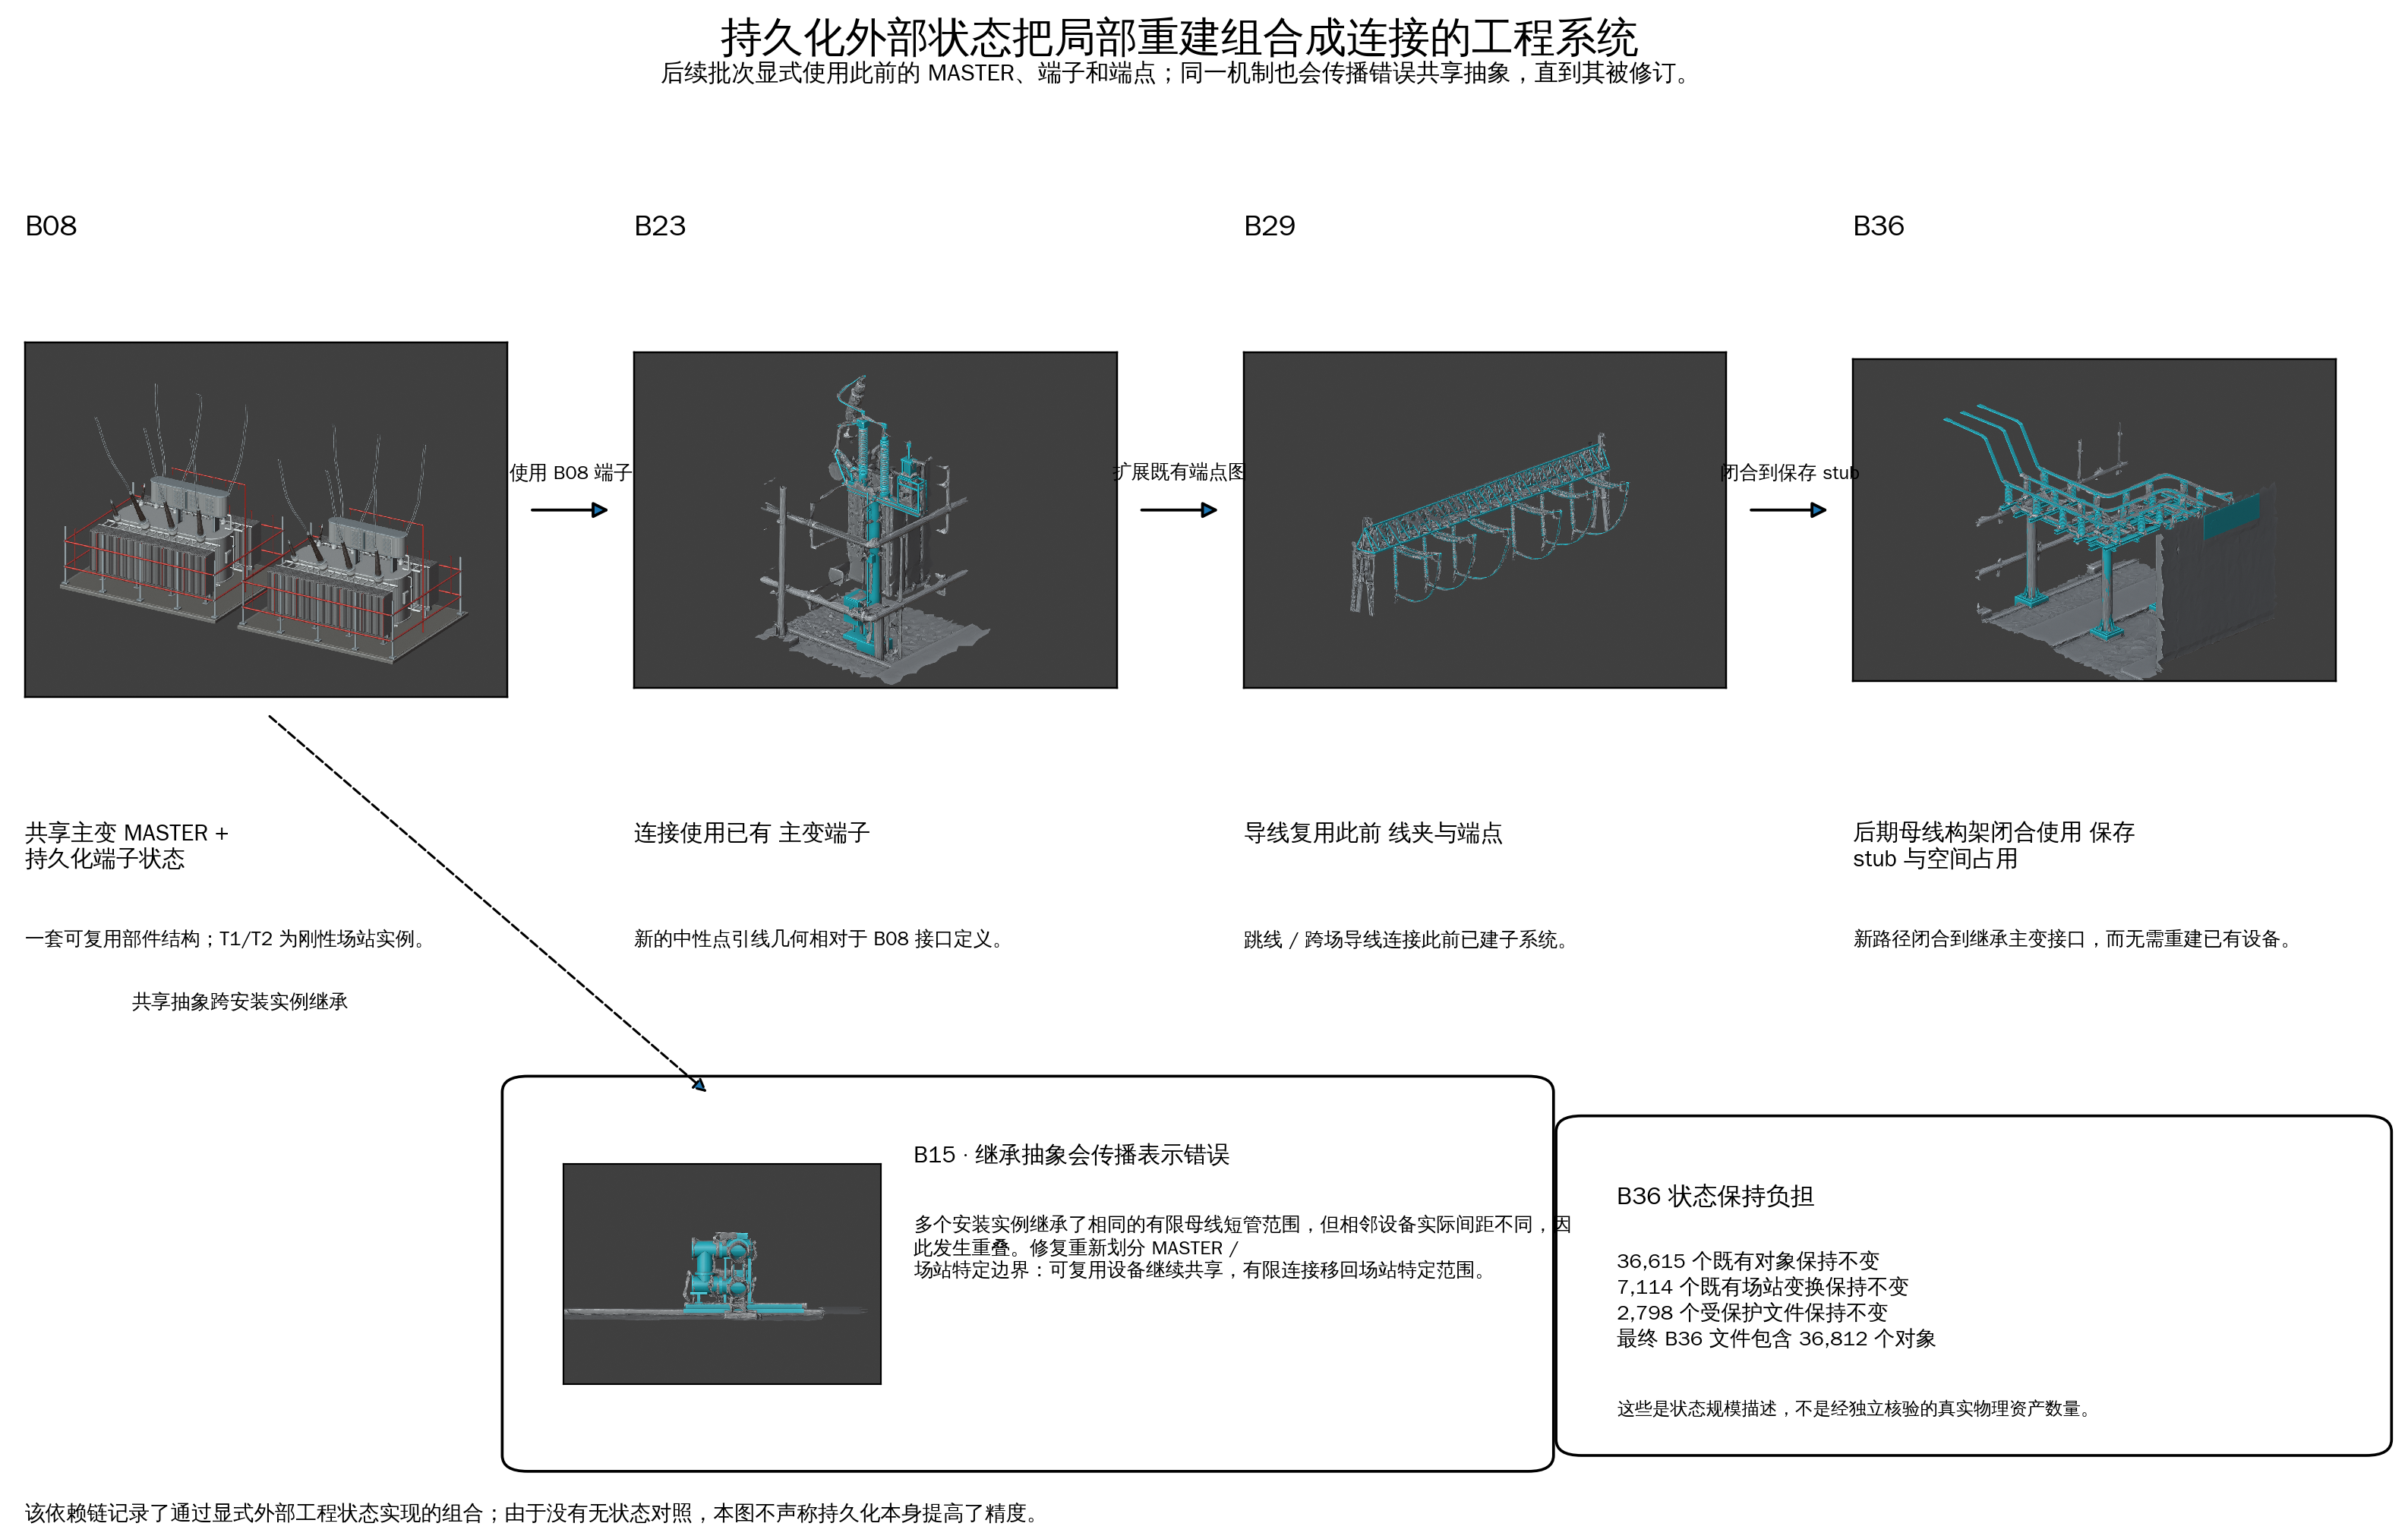
\includegraphics[width=\textwidth,height=0.3\textheight,keepaspectratio]{figures/fig05_persistent_state_dependency_b01_b36_zh.png}
\caption{从 B08 主变状态经 B23、B29 的连接一直延伸到 B36 场站闭合的显式跨批次依赖链。B15 分支展示了对应风险：共享表示中的不合适有限范围会持续传播，直到 MASTER/场站特定边界被修订。B36 的保持数量用于描述工程状态负担，并不是独立核验的物理资产数量。}
\label{fig:persistence}
\end{figure*}

这些证据只支持一个比``记忆提高重建效果''更窄的结论。本文没有无状态对照实验，也没有量化持久化状态带来的精度或效率收益。B01--B36
真正记录的是该工作流实现长时程重建的机制：后续任务作用于一个显式的外部工程世界，该世界包含先前资产、变换、端口和连接，而验证器在加入新几何时保护这些既有状态。同一个机制也使上游抽象选择成为下游问题的一部分。从这个意义上说，持久化改变了重建对象本身：它不再是一串彼此隔离的资产，而是一个累积形成的工程系统。

\hypertarget{ux8ba8ux8bba}{%
\section{讨论}\label{ux8ba8ux8bba}}

\hypertarget{ux901aux7528ux63a8ux7406ux6a21ux578bux8d21ux732eux4e86ux4ec0ux4e48}{%
\subsection{通用推理模型贡献了什么}\label{ux901aux7528ux63a8ux7406ux6a21ux578bux8d21ux732eux4e86ux4ec0ux4e48}}

B01--B36
的记录支持一种相对具体的角色定位：通用推理最有价值的环节，是工程问题本身需要被定义或修订的地方，例如选择比较域、判断哪些几何可以跨安装位置复用、选择路径表示、识别相关端口与线路径，或者根据未解释场景证据选择下一个重建区域。数值拟合与验收仍由模型外部的显式几何代码和验证器完成。这个分工对于解释结果很重要。较低的残差或较小的端点间隙，只能说明所选择的程序产生了几何上一致的结果；它并不能说明语言模型直接进行了高精度数值优化。

纵向记录还表明，模型可观察到的角色是在扩展，而不是简单从``低层''推理转向``高层''推理。后期土建和集成批次中依然保留测量。真正发生变化的是测量周围需要被显式表示的关系数量。重复设备引入不变性与安装范围，连接系统引入已有部件之间的关系约束，而场站闭合则增加场景级遗漏与兼容性检查。因此，通用模型在这一场景中的价值，在于通过同一个程序化接口形成并修订异构操作，而不是用一个统一学习模型替代专用几何方法。

\hypertarget{ux4e3aux4ec0ux4e48ux663eux5f0fux5de5ux5177ux4e0eux9a8cux8bc1ux5c5eux4e8eux65b9ux6cd5ux672cux8eab}{%
\subsection{为什么显式工具与验证属于方法本身}\label{ux4e3aux4ec0ux4e48ux663eux5f0fux5de5ux5177ux4e0eux9a8cux8bc1ux5c5eux4e8eux65b9ux6cd5ux672cux8eab}}

本文结果依赖于一个重要前提：模型决策被外部化为可执行工件。B01/B02
保留了失败比较以及重新定义后的测量域，而不是隐藏最初筛查失败；B15
保存了产生重叠的共享短管表示，并记录其向场站特定有限几何的修订；B23
也保留了初始表示无法解释观测轨迹之后的连续几何修订。保留这些修订，使当前假设与物理证据之间的不一致能够被检查和追溯。

这一点之所以重要，还因为同一个摄影测量参考可以支持不同类型的检查。对于拟合墙体或圆柱，有限表面残差是有意义的，但它不能证明导线端点连续、路径完整，也不能证明既有场景状态保持。反过来，端点检查可以通过，但其周围源区域仍可能包含尚未解释的分支或附件。因此，任务特定验证器编码的是不同的验收条件，而不是逼近一个隐藏的全局分数。由此形成的系统更接近真实工程工作流：推理层提出显式操作，专用程序判断相应几何条件是否真正满足。

\hypertarget{ux6301ux4e45ux5316ux72b6ux6001ux540cux65f6ux6539ux53d8ux80fdux529bux8fb9ux754cux548cux98ceux9669}{%
\subsection{持久化状态同时改变能力边界和风险}\label{ux6301ux4e45ux5316ux72b6ux6001ux540cux65f6ux6539ux53d8ux80fdux529bux8fb9ux754cux548cux98ceux9669}}

持久化外部状态使后续批次面对的是一个已经工程化的世界，而不是空白场景。B23
可以把新引线终止在 B08 的已有端子上，B29
可以把新导线接到此前的悬垂端与主变接口，B36
则可以把新母线闭合到已经保存的主变
stub。正因为一个批次的输出会成为另一个批次的输入结构，这些依赖才使场站级组合在该工作流中成为可能。

同一个机制也会使表示错误具有非局部影响。B15
表明，如果一个本应场站特定的有限短管被放进共享抽象，不合适的几何会传播到多个安装实例。修复时需要改变复用边界，而不是简单移动一个对象。因此，持久化状态应被视为重建问题的一部分，而不仅仅是存储方式。它提供组合杠杆，同时也要求来源记录、限定范围验证，以及在不破坏已验收历史的前提下修订继承抽象的能力。

\hypertarget{ux5c40ux9650ux6027ux4e0eux6709ux6548ux6027ux5a01ux80c1}{%
\subsection{局限性与有效性威胁}\label{ux5c40ux9650ux6027ux4e0eux6709ux6548ux6027ux5a01ux80c1}}

当前证据来自一座变电站和一套由项目负责人确认的 GPT-6 Astra/Codex
配置的纵向现场记录。本文没有在同一工具框架下运行匹配的替代规划器或模型，因此不能据此证明模型优越性，也不能隔离哪些行为能够迁移到其他语言模型。任务序列是历史形成且状态相关的，并未由统一难度变量进行实验控制。算子分析来自保存脚本与文件工件，它描述记录中的工作流，但不是标准化动作遥测。

几何证据本身也有相应边界。多数数值比较使用了同时参与建模决策的同一个配准摄影测量重建，因此它们测量的是在给定比较域下与该参考的一致性，而不是独立测量精度。部分检查在同一个空间相关重建中使用奇偶面划分，也不应被解释为独立测量。完整场站没有独立测量参考，可见室外模型也不能证明隐藏、室内或地下结构的完整性。

人工输入同样会影响轨迹。B08
的复用建立在用户明确授权``两台主变部件配置等价''的基础上，复核也可能暴露遗漏或歧义结构。因此，该系统是``智能体驱动、人工可引导''的，而不是完全自主。最后，历史工件保存了程序、计划、诊断与修订结果，却没有保存模型的私有推理过程。本文关于模型的结论仅限于可观察决策和保存工件。

\hypertarget{ux540eux7eedux53d7ux63a7ux5b9eux9a8c}{%
\subsection{后续受控实验}\label{ux540eux7eedux53d7ux63a7ux5b9eux9a8c}}

更强的比较研究应固定工程执行框架，只改变少量受控因素。最有信息量的下一步，是在本文三个结构性转变中选择代表任务，运行匹配的替代模型：包括局部比较域形成、可复用范围修订、连接路径表示以及后期受既有状态约束的插入。第二项扩展可以针对少量设备和连接获取独立测量数据，从而把任务局部几何精度与外部参考进行比较。第三项扩展是在第二个站点复现实验，以检验本文观察到的算子模式是否特定于当前变电站。最后，如果未来能够显式记录模型调用、人工介入、运行时间和工具调用，就可以比当前基于历史工件的回溯更精确地分析成本、自主性和决策来源。

\hypertarget{ux7ed3ux8bba}{%
\section{结论}\label{ux7ed3ux8bba}}

B01--B36
记录了一种持久化、程序化的部件级工业重建方法：通用推理模型负责形成和修订显式几何操作，确定性工具负责数值估计与验证。其主要纵向结果是：随着重建依赖关系增加，算子集合不断扩展。局部比较与拟合始终存在，而后期任务逐步加入可复用范围、关系几何、剩余工作选择以及与既有工程场景兼容性的决策。持久化外部工程状态使已验收部件和接口能够在后续任务中被复用，但
B15
同时表明，错误的共享抽象也会沿同一机制传播。本文由此提供的是一个单站点长时程现场重建的系统性描述，而不是模型比较基准。未来仍需在相同执行框架下进行匹配的替代模型实验、针对部分结构获取独立测量参考，并在第二个站点进行复现，以检验一般性与比较性能。
\balance
\small
\bibliographystyle{unsrtnat}
\bibliography{references}
\end{document}
